\documentclass[11pt]{article}
\usepackage[textwidth=18.0cm, textheight=23.0cm, top=2.0cm]{geometry}
\usepackage{pst-all}
\usepackage{amssymb}
\usepackage{tikz}
\usepackage{underscore}\begin{document}
\pagestyle{empty}


ClassName: \underline{\textbf{Class_08.2bp-17}}
\par
BinSize: \underline{\textbf{100 × 100}}
\par
ReduceSize: \underline{\textbf{100 × 100}}
\par
TypeNum: \underline{\textbf{40}}
\par
Num: \underline{\textbf{40}}
\par
OutS: \underline{\textbf{110000}}
\par
InS: \underline{\textbf{91811}}
\par
Rate: \underline{\textbf{0.835}}
\par
UB: \underline{\textbf{11}}
\par
LB0: \underline{\textbf{11}}
\par
LB: \underline{\textbf{11}}
\par
LBWithCut: \underline{\textbf{11}}
\par
NodeCut: \underline{\textbf{0}}
\par
ExtendedNodeCnt: \underline{\textbf{1}}
\par
GenNodeCnt: \underline{\textbf{1}}
\par
PrimalNode: \underline{\textbf{0}}
\par
ColumnCount: \underline{\textbf{11}}
\par
TotalCutCount: \underline{\textbf{0}}
\par
RootCutCount: \underline{\textbf{0}}
\par
LPSolverCnt: \underline{\textbf{1}}
\par
PricingSolverCnt: \underline{\textbf{0}}
\par
BranchAndBoundNum: \underline{\textbf{1}}
\par
isOpt: \underline{\textbf{true}}
\par
TimeOnInitSolution: \underline{\textbf{600.000 s}}
\par
TimeOnPrimal: \underline{\textbf{0.000 s}}
\par
TimeOnPricing: \underline{\textbf{0.000 s}}
\par
TimeOnRmp: \underline{\textbf{0.047 s}}
\par
TotalTime: \underline{\textbf{600.328 s}}
\par
\newpage


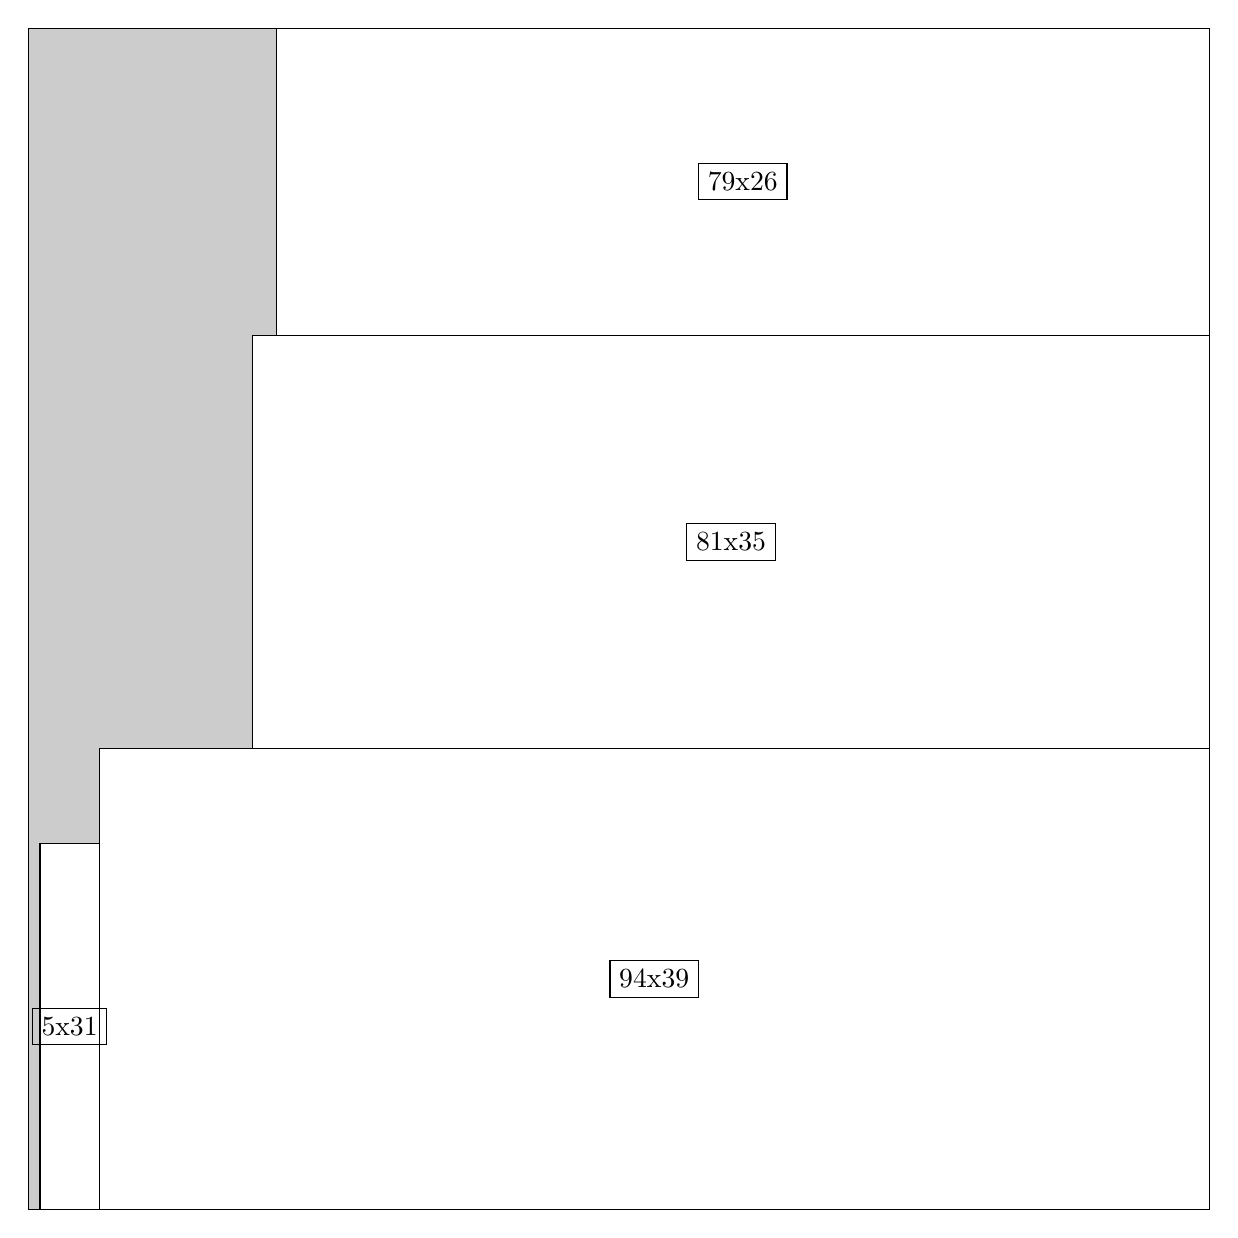
\begin{tikzpicture}[shorten >=1pt,scale=1.0,every node/.style={scale=1.0},->]
\tikzstyle{vertex}=[circle,fill=black!25,minimum size=14pt,inner sep=0pt]
\filldraw[fill=gray!40!white, draw=black] (0,0) rectangle (15.0,15.0);
\foreach \name/\x/\y/\w/\h in {94x39/0.8999999999999999/0.0/14.1/5.85,5x31/0.15/0.0/0.75/4.6499999999999995,81x35/2.85/5.85/12.15/5.25,79x26/3.15/11.1/11.85/3.9}
\filldraw[fill=white!40!white, draw=black] (\x,\y) rectangle node[draw] (\name) {\name} ++(\w,\h);
\end{tikzpicture}


w =94 , h =39 , x =6 , y =0 , v =3666
\par
w =5 , h =31 , x =1 , y =0 , v =155
\par
w =81 , h =35 , x =19 , y =39 , v =2835
\par
w =79 , h =26 , x =21 , y =74 , v =2054
\par
\newpage


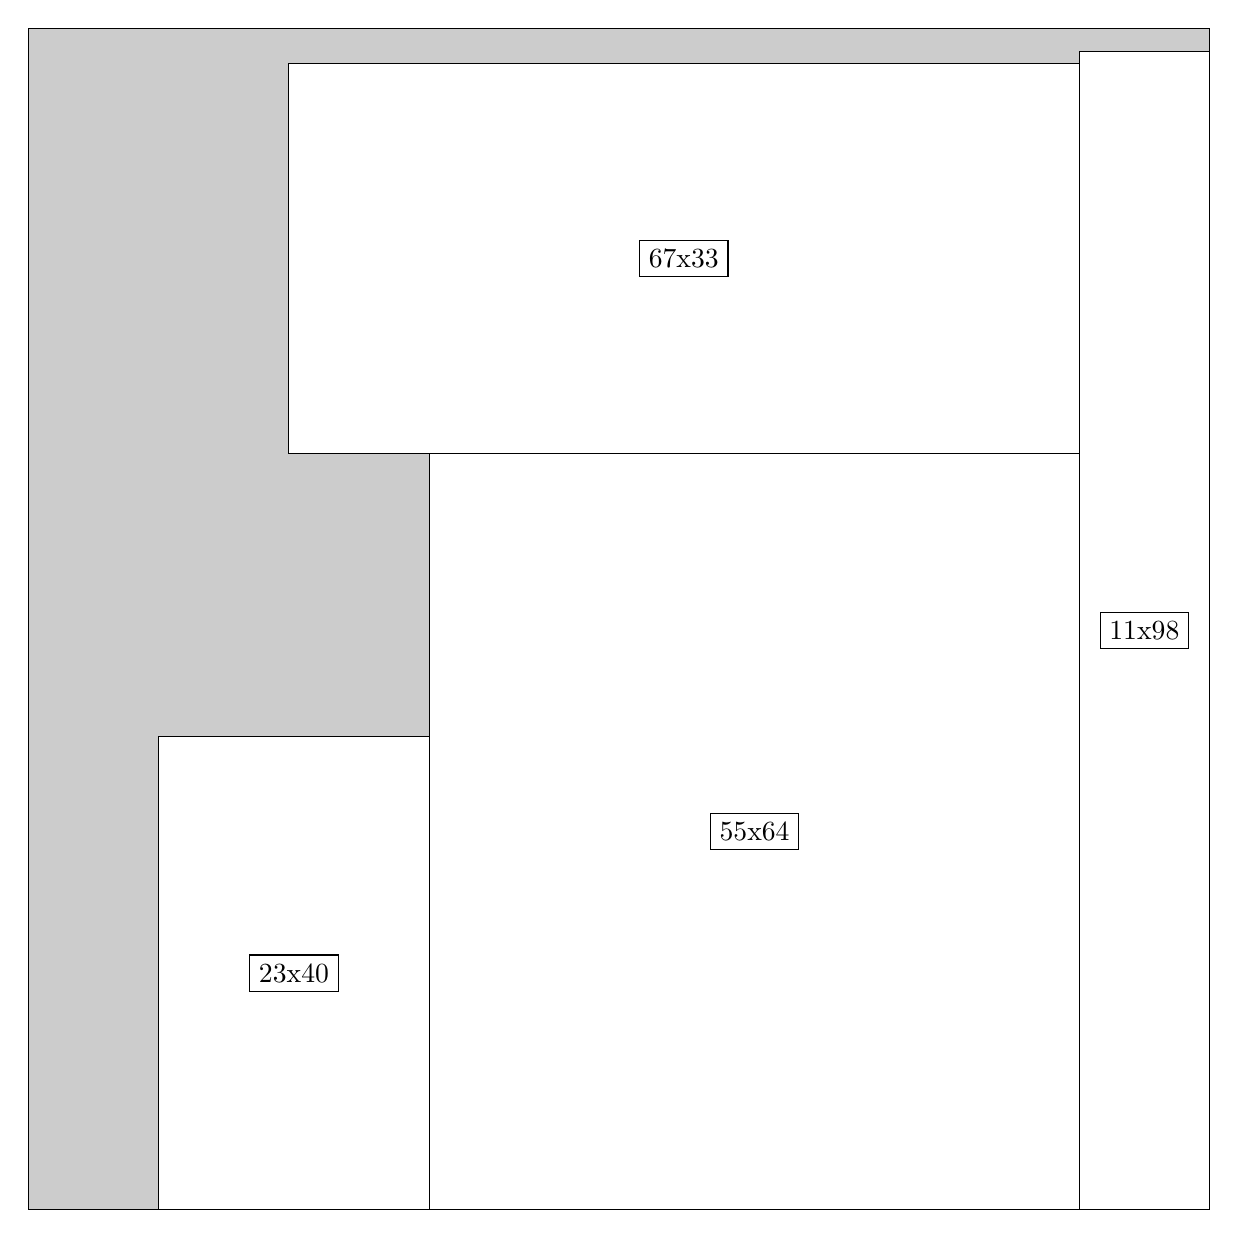
\begin{tikzpicture}[shorten >=1pt,scale=1.0,every node/.style={scale=1.0},->]
\tikzstyle{vertex}=[circle,fill=black!25,minimum size=14pt,inner sep=0pt]
\filldraw[fill=gray!40!white, draw=black] (0,0) rectangle (15.0,15.0);
\foreach \name/\x/\y/\w/\h in {11x98/13.35/0.0/1.65/14.7,55x64/5.1/0.0/8.25/9.6,23x40/1.65/0.0/3.4499999999999997/6.0,67x33/3.3/9.6/10.049999999999999/4.95}
\filldraw[fill=white!40!white, draw=black] (\x,\y) rectangle node[draw] (\name) {\name} ++(\w,\h);
\end{tikzpicture}


w =11 , h =98 , x =89 , y =0 , v =1078
\par
w =55 , h =64 , x =34 , y =0 , v =3520
\par
w =23 , h =40 , x =11 , y =0 , v =920
\par
w =67 , h =33 , x =22 , y =64 , v =2211
\par
\newpage


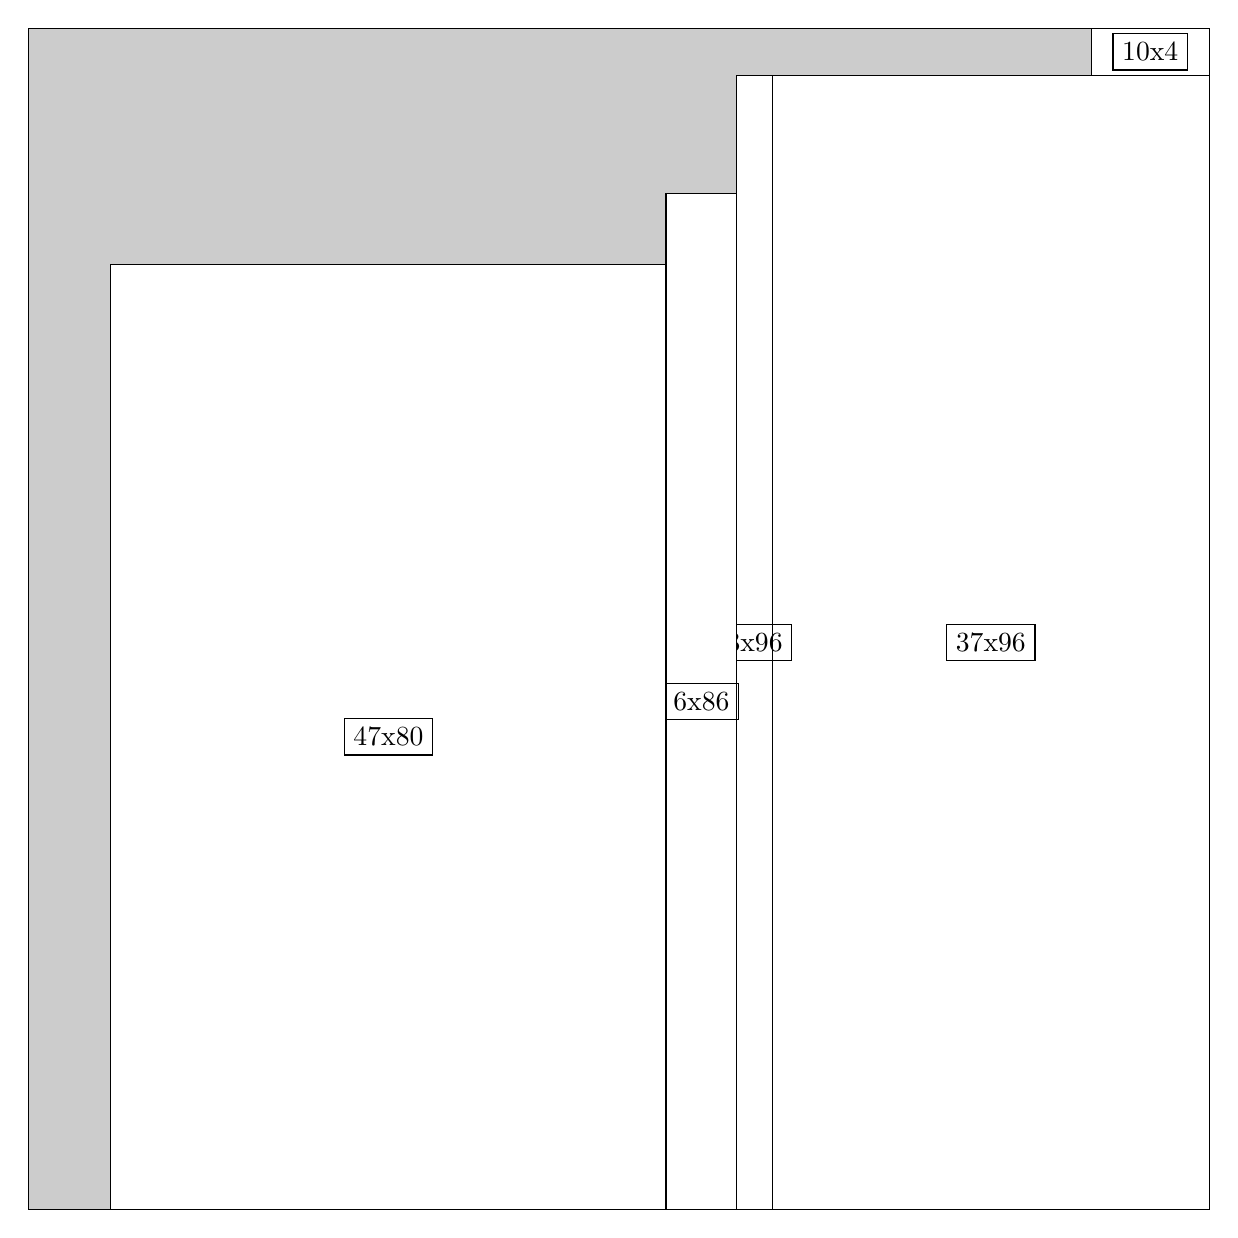
\begin{tikzpicture}[shorten >=1pt,scale=1.0,every node/.style={scale=1.0},->]
\tikzstyle{vertex}=[circle,fill=black!25,minimum size=14pt,inner sep=0pt]
\filldraw[fill=gray!40!white, draw=black] (0,0) rectangle (15.0,15.0);
\foreach \name/\x/\y/\w/\h in {37x96/9.45/0.0/5.55/14.399999999999999,10x4/13.5/14.399999999999999/1.5/0.6,3x96/9.0/0.0/0.44999999999999996/14.399999999999999,6x86/8.1/0.0/0.8999999999999999/12.9,47x80/1.05/0.0/7.05/12.0}
\filldraw[fill=white!40!white, draw=black] (\x,\y) rectangle node[draw] (\name) {\name} ++(\w,\h);
\end{tikzpicture}


w =37 , h =96 , x =63 , y =0 , v =3552
\par
w =10 , h =4 , x =90 , y =96 , v =40
\par
w =3 , h =96 , x =60 , y =0 , v =288
\par
w =6 , h =86 , x =54 , y =0 , v =516
\par
w =47 , h =80 , x =7 , y =0 , v =3760
\par
\newpage


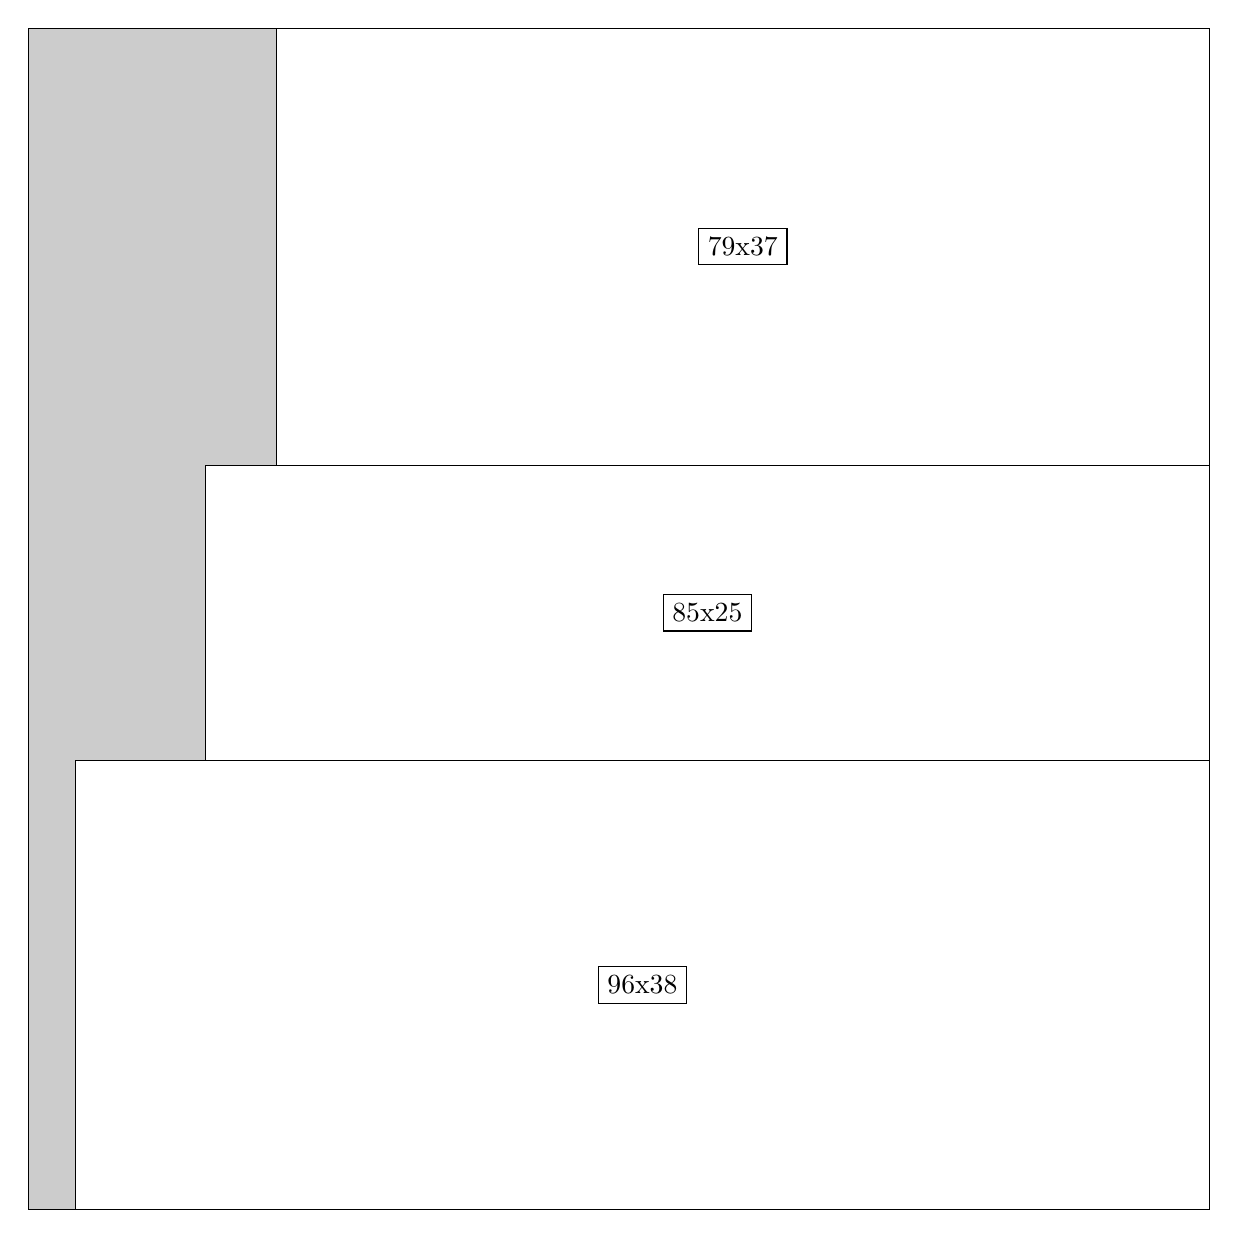
\begin{tikzpicture}[shorten >=1pt,scale=1.0,every node/.style={scale=1.0},->]
\tikzstyle{vertex}=[circle,fill=black!25,minimum size=14pt,inner sep=0pt]
\filldraw[fill=gray!40!white, draw=black] (0,0) rectangle (15.0,15.0);
\foreach \name/\x/\y/\w/\h in {96x38/0.6/0.0/14.399999999999999/5.7,85x25/2.25/5.7/12.75/3.75,79x37/3.15/9.45/11.85/5.55}
\filldraw[fill=white!40!white, draw=black] (\x,\y) rectangle node[draw] (\name) {\name} ++(\w,\h);
\end{tikzpicture}


w =96 , h =38 , x =4 , y =0 , v =3648
\par
w =85 , h =25 , x =15 , y =38 , v =2125
\par
w =79 , h =37 , x =21 , y =63 , v =2923
\par
\newpage


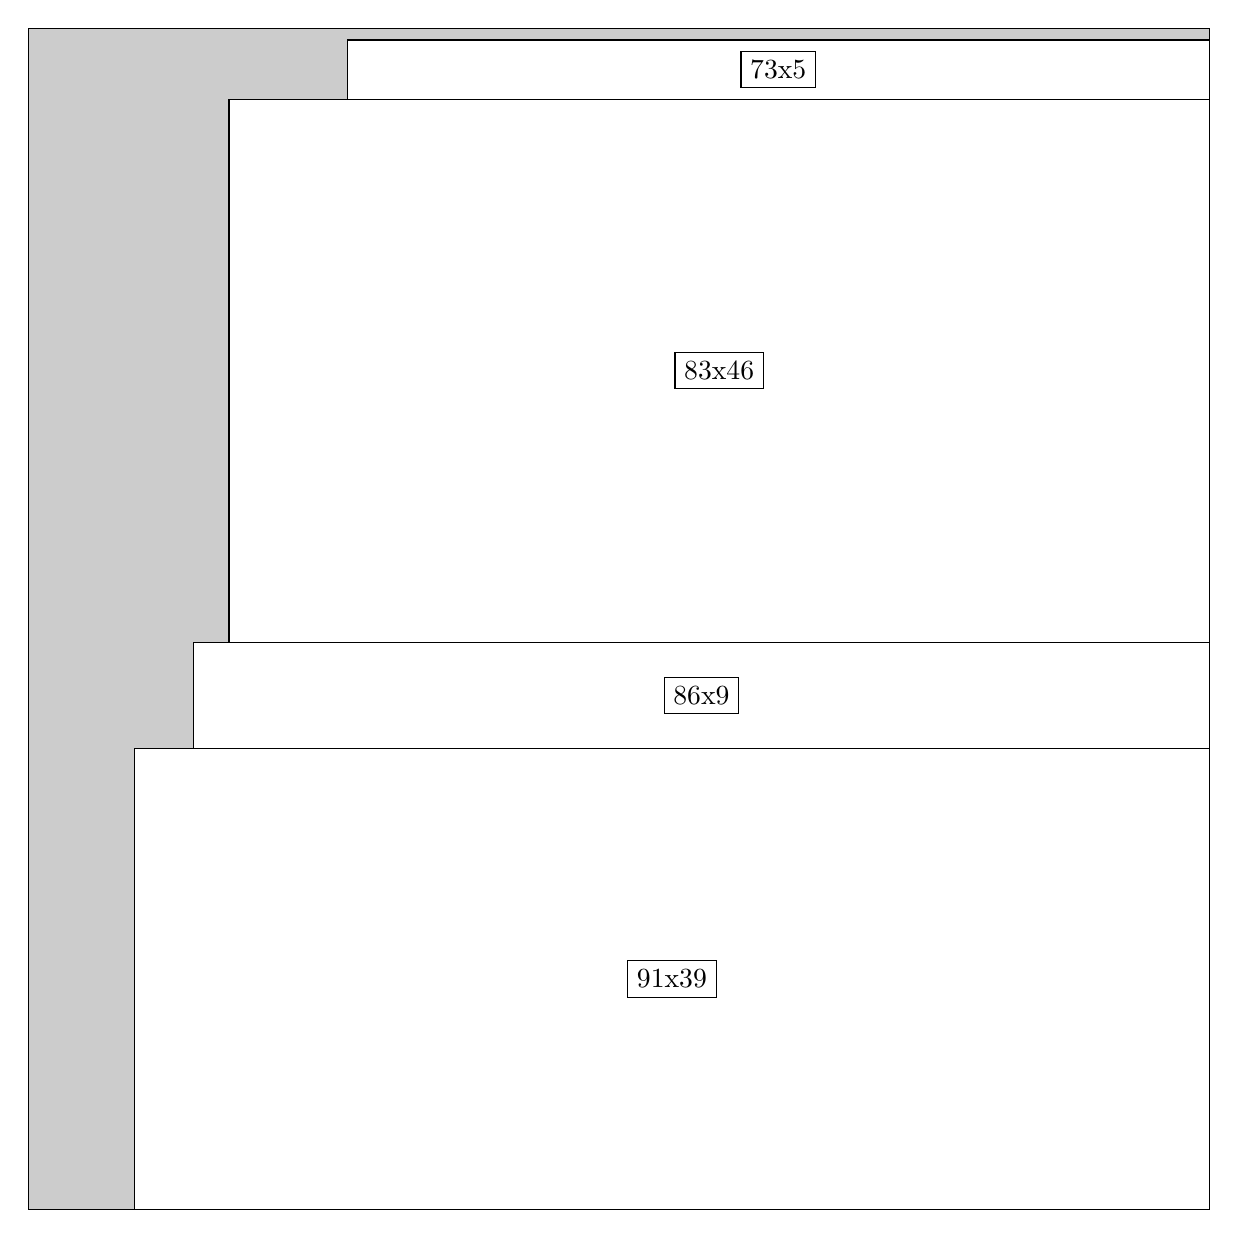
\begin{tikzpicture}[shorten >=1pt,scale=1.0,every node/.style={scale=1.0},->]
\tikzstyle{vertex}=[circle,fill=black!25,minimum size=14pt,inner sep=0pt]
\filldraw[fill=gray!40!white, draw=black] (0,0) rectangle (15.0,15.0);
\foreach \name/\x/\y/\w/\h in {91x39/1.3499999999999999/0.0/13.65/5.85,86x9/2.1/5.85/12.9/1.3499999999999999,83x46/2.55/7.199999999999999/12.45/6.8999999999999995,73x5/4.05/14.1/10.95/0.75}
\filldraw[fill=white!40!white, draw=black] (\x,\y) rectangle node[draw] (\name) {\name} ++(\w,\h);
\end{tikzpicture}


w =91 , h =39 , x =9 , y =0 , v =3549
\par
w =86 , h =9 , x =14 , y =39 , v =774
\par
w =83 , h =46 , x =17 , y =48 , v =3818
\par
w =73 , h =5 , x =27 , y =94 , v =365
\par
\newpage


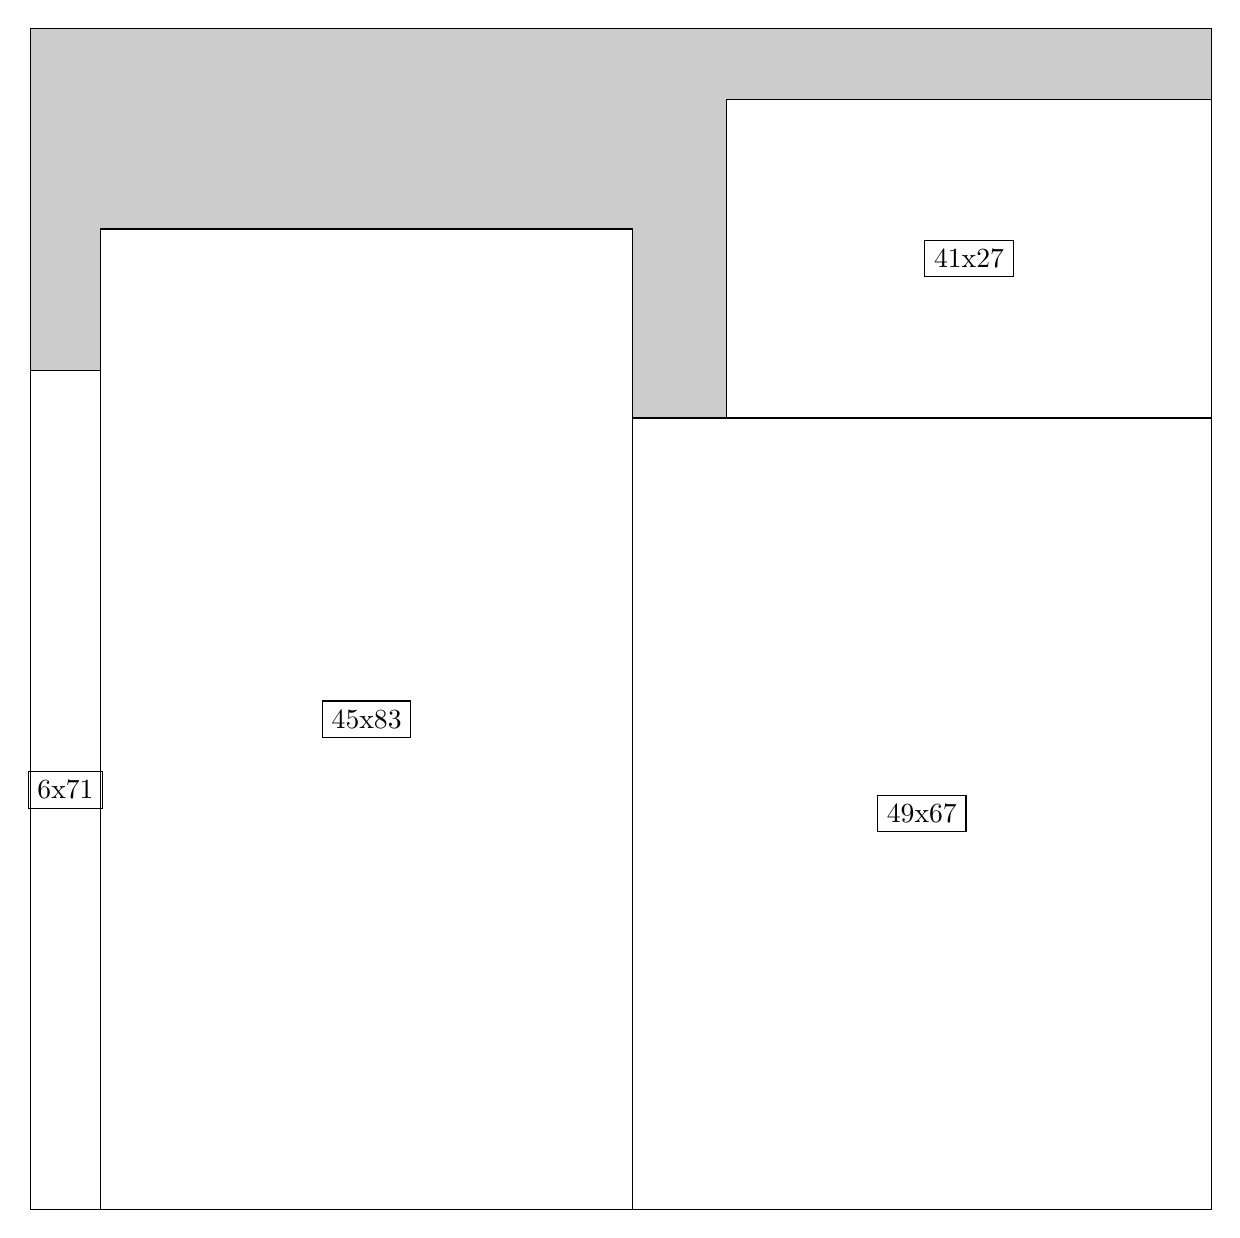
\begin{tikzpicture}[shorten >=1pt,scale=1.0,every node/.style={scale=1.0},->]
\tikzstyle{vertex}=[circle,fill=black!25,minimum size=14pt,inner sep=0pt]
\filldraw[fill=gray!40!white, draw=black] (0,0) rectangle (15.0,15.0);
\foreach \name/\x/\y/\w/\h in {49x67/7.6499999999999995/0.0/7.35/10.049999999999999,41x27/8.85/10.049999999999999/6.1499999999999995/4.05,45x83/0.8999999999999999/0.0/6.75/12.45,6x71/0.0/0.0/0.8999999999999999/10.65}
\filldraw[fill=white!40!white, draw=black] (\x,\y) rectangle node[draw] (\name) {\name} ++(\w,\h);
\end{tikzpicture}


w =49 , h =67 , x =51 , y =0 , v =3283
\par
w =41 , h =27 , x =59 , y =67 , v =1107
\par
w =45 , h =83 , x =6 , y =0 , v =3735
\par
w =6 , h =71 , x =0 , y =0 , v =426
\par
\newpage


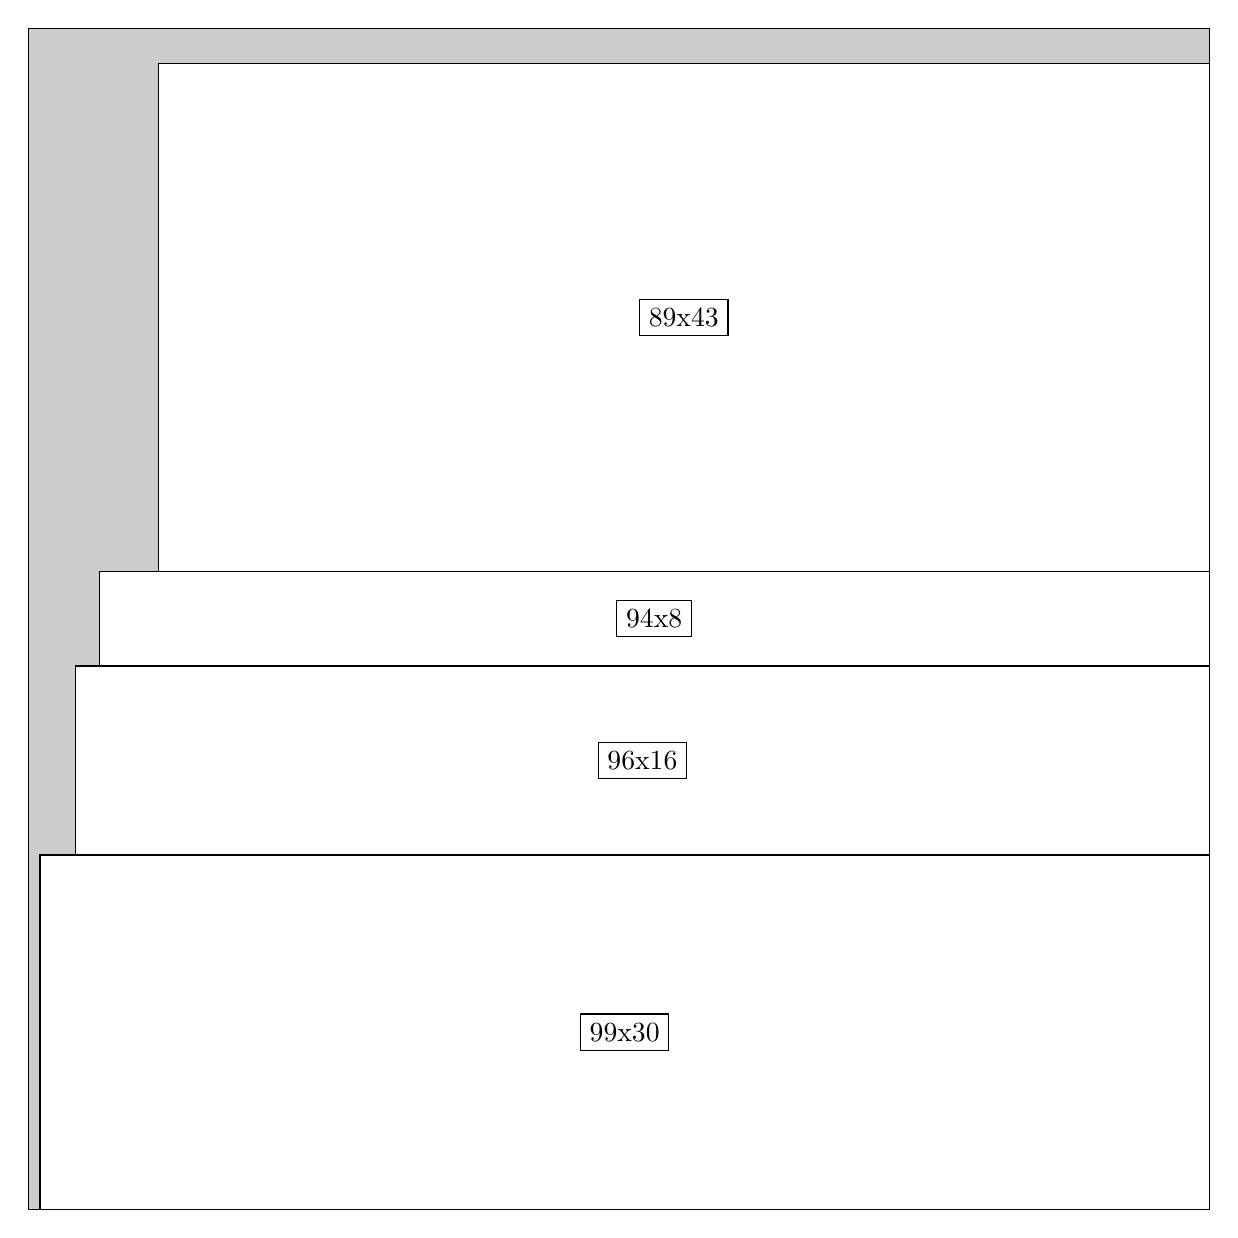
\begin{tikzpicture}[shorten >=1pt,scale=1.0,every node/.style={scale=1.0},->]
\tikzstyle{vertex}=[circle,fill=black!25,minimum size=14pt,inner sep=0pt]
\filldraw[fill=gray!40!white, draw=black] (0,0) rectangle (15.0,15.0);
\foreach \name/\x/\y/\w/\h in {99x30/0.15/0.0/14.85/4.5,96x16/0.6/4.5/14.399999999999999/2.4,94x8/0.8999999999999999/6.8999999999999995/14.1/1.2,89x43/1.65/8.1/13.35/6.45}
\filldraw[fill=white!40!white, draw=black] (\x,\y) rectangle node[draw] (\name) {\name} ++(\w,\h);
\end{tikzpicture}


w =99 , h =30 , x =1 , y =0 , v =2970
\par
w =96 , h =16 , x =4 , y =30 , v =1536
\par
w =94 , h =8 , x =6 , y =46 , v =752
\par
w =89 , h =43 , x =11 , y =54 , v =3827
\par
\newpage


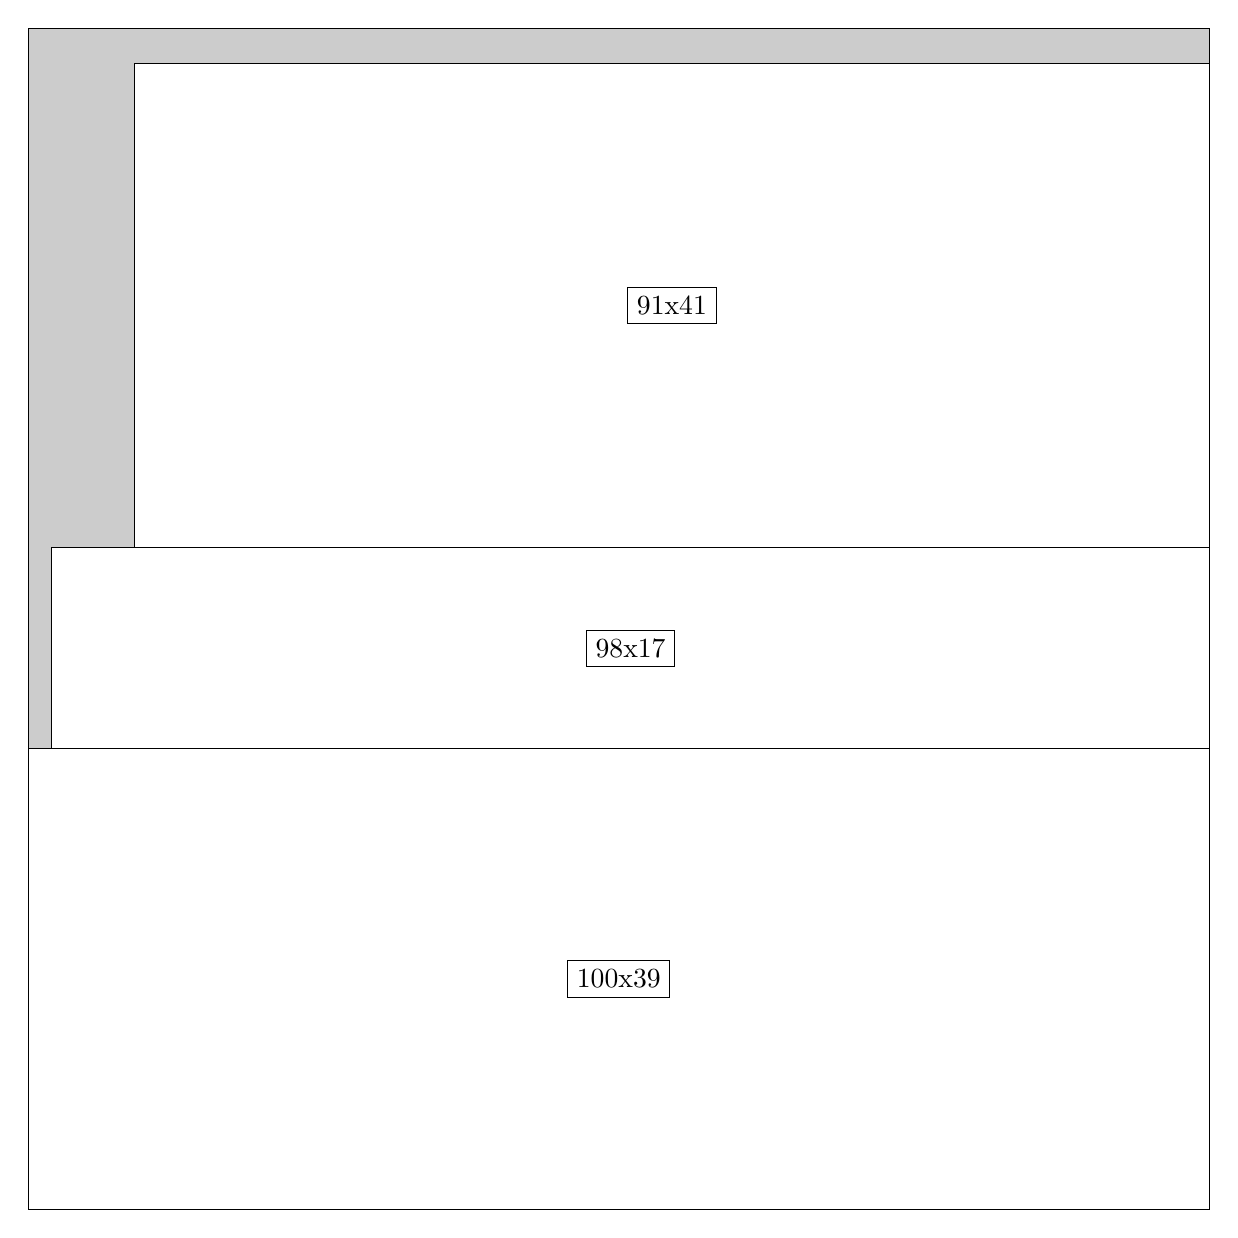
\begin{tikzpicture}[shorten >=1pt,scale=1.0,every node/.style={scale=1.0},->]
\tikzstyle{vertex}=[circle,fill=black!25,minimum size=14pt,inner sep=0pt]
\filldraw[fill=gray!40!white, draw=black] (0,0) rectangle (15.0,15.0);
\foreach \name/\x/\y/\w/\h in {100x39/0.0/0.0/15.0/5.85,98x17/0.3/5.85/14.7/2.55,91x41/1.3499999999999999/8.4/13.65/6.1499999999999995}
\filldraw[fill=white!40!white, draw=black] (\x,\y) rectangle node[draw] (\name) {\name} ++(\w,\h);
\end{tikzpicture}


w =100 , h =39 , x =0 , y =0 , v =3900
\par
w =98 , h =17 , x =2 , y =39 , v =1666
\par
w =91 , h =41 , x =9 , y =56 , v =3731
\par
\newpage


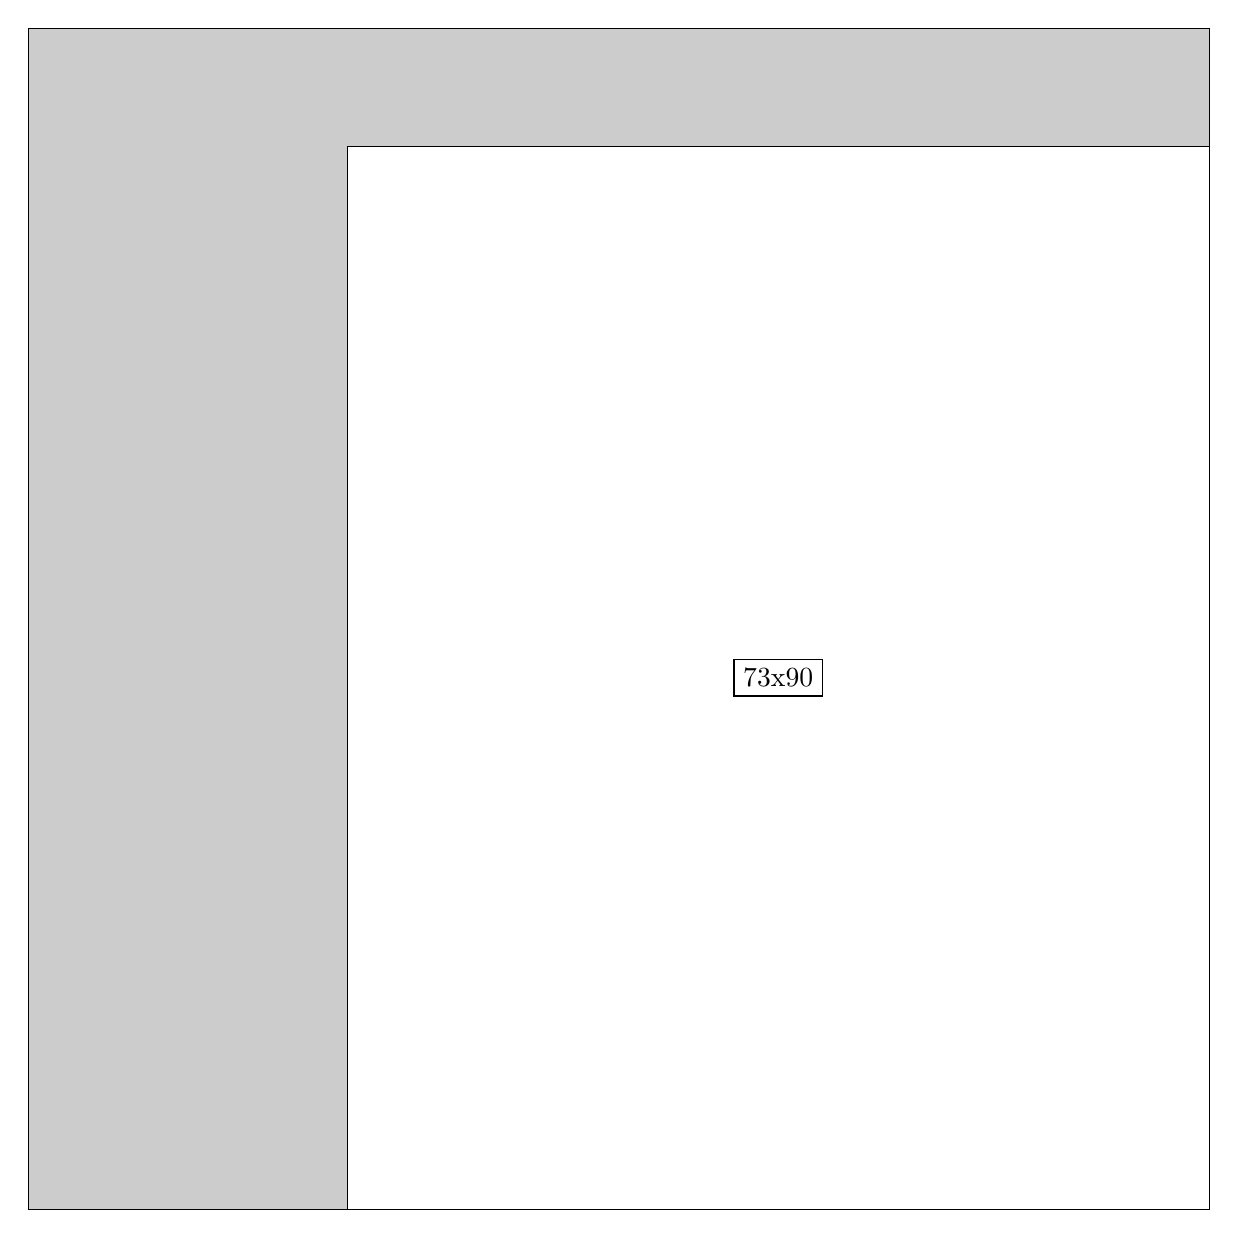
\begin{tikzpicture}[shorten >=1pt,scale=1.0,every node/.style={scale=1.0},->]
\tikzstyle{vertex}=[circle,fill=black!25,minimum size=14pt,inner sep=0pt]
\filldraw[fill=gray!40!white, draw=black] (0,0) rectangle (15.0,15.0);
\foreach \name/\x/\y/\w/\h in {73x90/4.05/0.0/10.95/13.5}
\filldraw[fill=white!40!white, draw=black] (\x,\y) rectangle node[draw] (\name) {\name} ++(\w,\h);
\end{tikzpicture}


w =73 , h =90 , x =27 , y =0 , v =6570
\par
\newpage


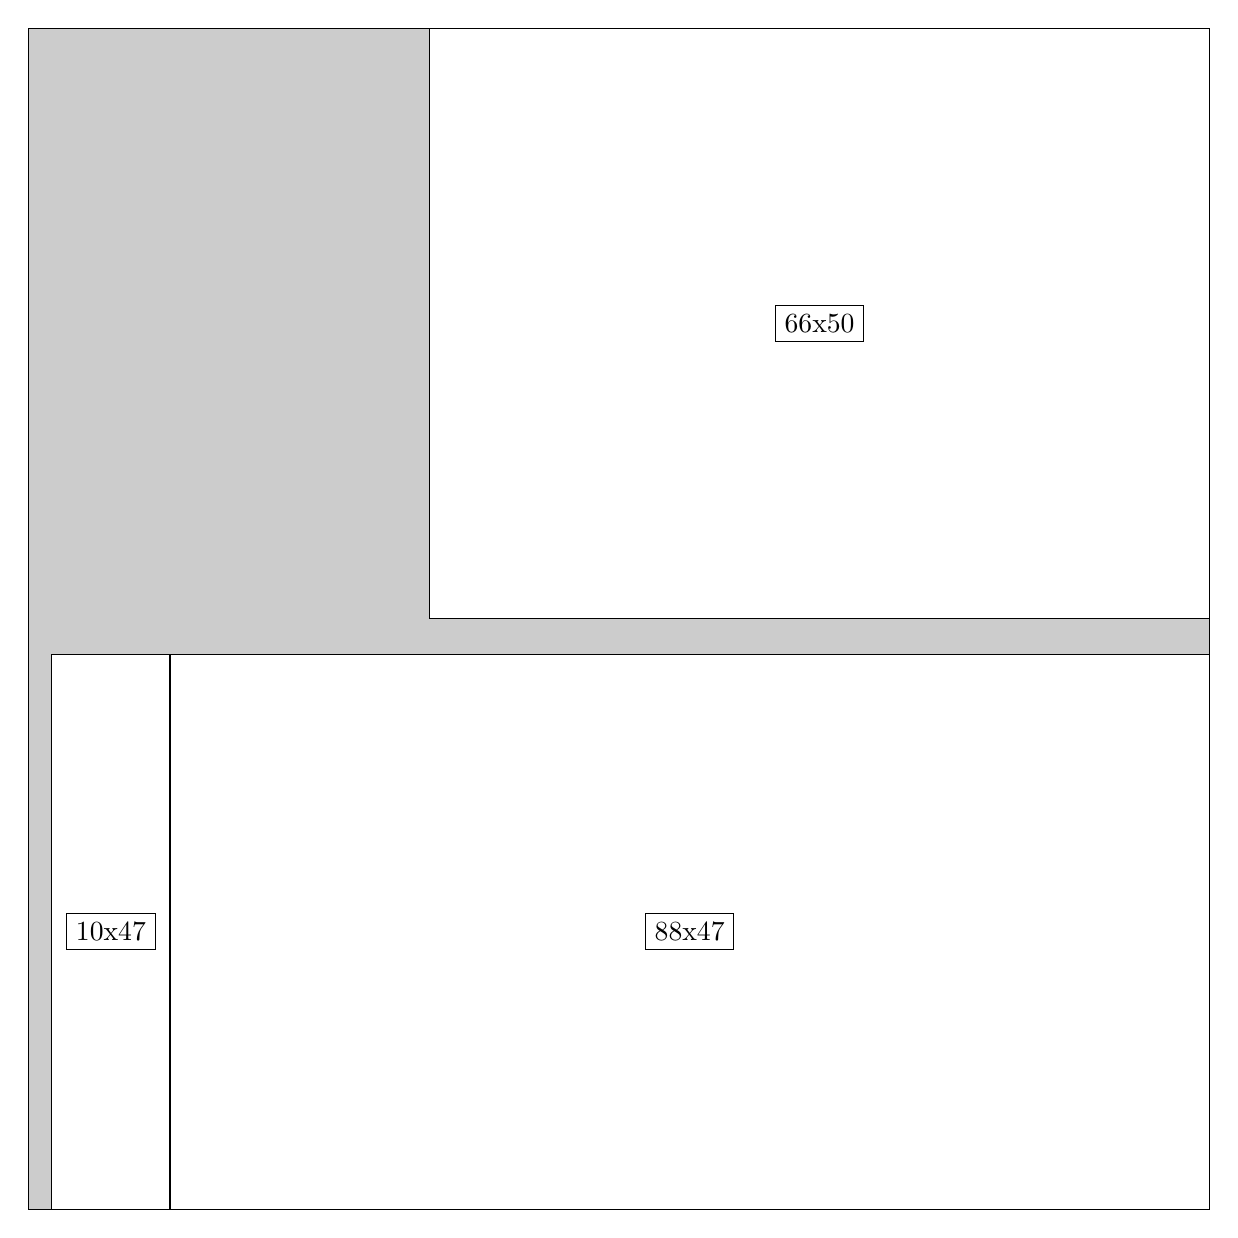
\begin{tikzpicture}[shorten >=1pt,scale=1.0,every node/.style={scale=1.0},->]
\tikzstyle{vertex}=[circle,fill=black!25,minimum size=14pt,inner sep=0pt]
\filldraw[fill=gray!40!white, draw=black] (0,0) rectangle (15.0,15.0);
\foreach \name/\x/\y/\w/\h in {88x47/1.7999999999999998/0.0/13.2/7.05,10x47/0.3/0.0/1.5/7.05,66x50/5.1/7.5/9.9/7.5}
\filldraw[fill=white!40!white, draw=black] (\x,\y) rectangle node[draw] (\name) {\name} ++(\w,\h);
\end{tikzpicture}


w =88 , h =47 , x =12 , y =0 , v =4136
\par
w =10 , h =47 , x =2 , y =0 , v =470
\par
w =66 , h =50 , x =34 , y =50 , v =3300
\par
\newpage


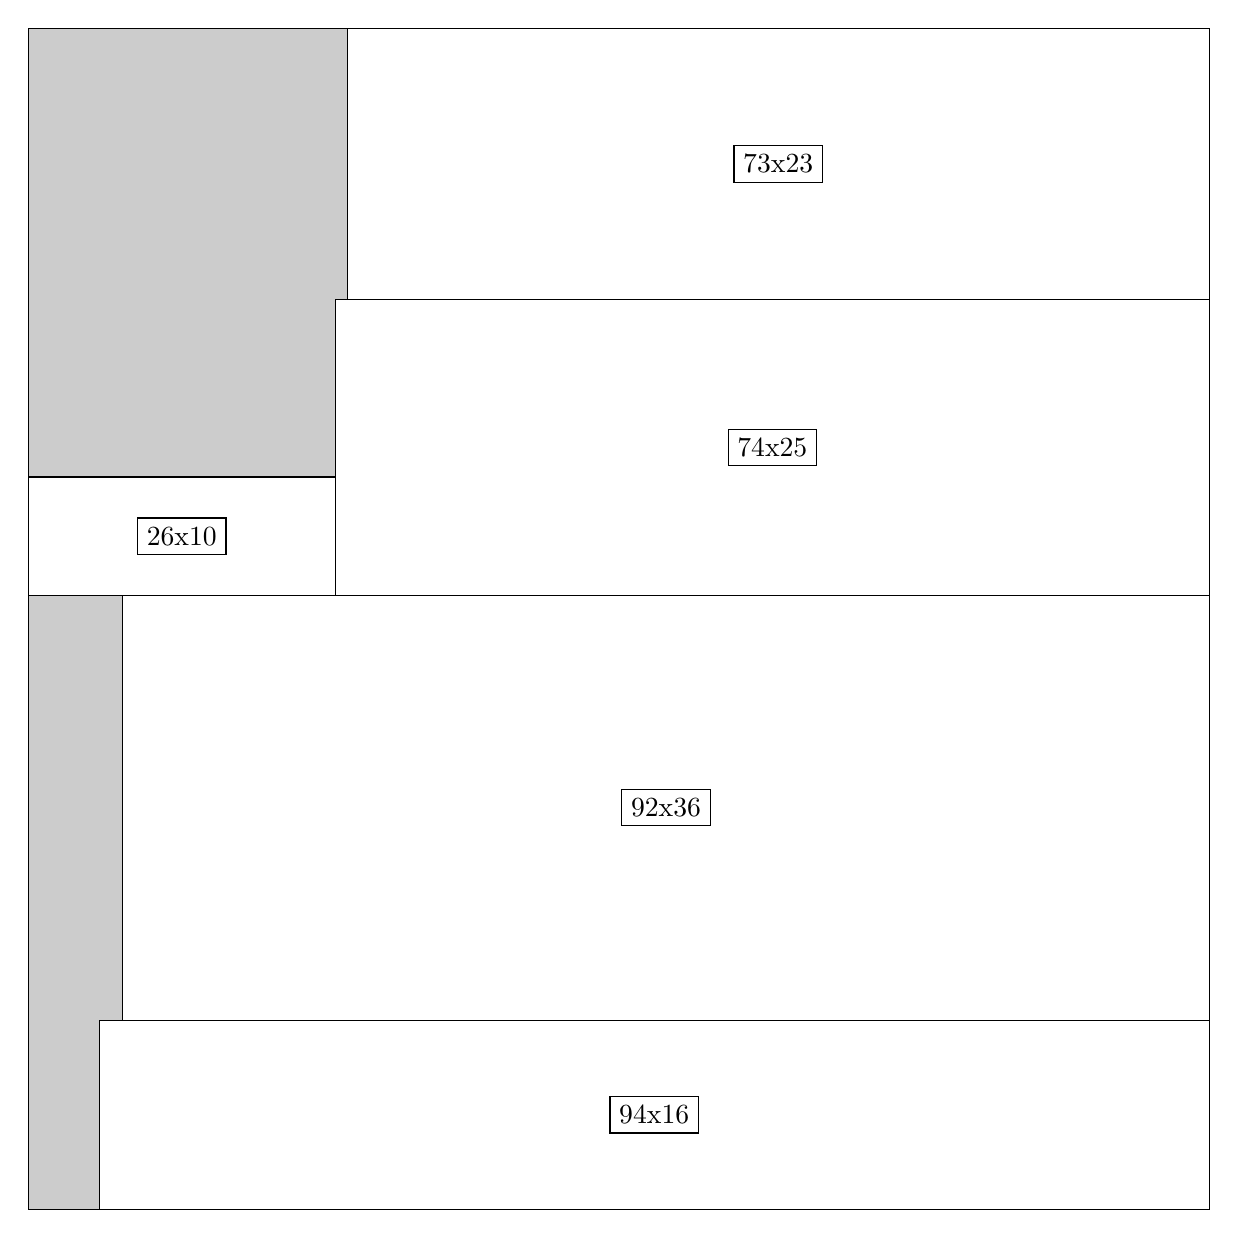
\begin{tikzpicture}[shorten >=1pt,scale=1.0,every node/.style={scale=1.0},->]
\tikzstyle{vertex}=[circle,fill=black!25,minimum size=14pt,inner sep=0pt]
\filldraw[fill=gray!40!white, draw=black] (0,0) rectangle (15.0,15.0);
\foreach \name/\x/\y/\w/\h in {94x16/0.8999999999999999/0.0/14.1/2.4,92x36/1.2/2.4/13.799999999999999/5.3999999999999995,74x25/3.9/7.8/11.1/3.75,26x10/0.0/7.8/3.9/1.5,73x23/4.05/11.549999999999999/10.95/3.4499999999999997}
\filldraw[fill=white!40!white, draw=black] (\x,\y) rectangle node[draw] (\name) {\name} ++(\w,\h);
\end{tikzpicture}


w =94 , h =16 , x =6 , y =0 , v =1504
\par
w =92 , h =36 , x =8 , y =16 , v =3312
\par
w =74 , h =25 , x =26 , y =52 , v =1850
\par
w =26 , h =10 , x =0 , y =52 , v =260
\par
w =73 , h =23 , x =27 , y =77 , v =1679
\par
\newpage


\end{document}